% Chapter 2

\chapter{The LHC and CMS experiment} % 
\section{The Large Hardon Collider}
\label{lhc_intro}
%LHC intro 
The LHC is a 27km circular circumference storage ring, accelerator and collider for 
both protons and Pb ions. It is situated in a stable environment in a tunnel 
100 metres underneath the Franco-Swiss boder near Geneva, Switzerland.
A double-ring synchotron, it is designed to collide proton-proton (p-p)
pairs with a centre of mass energy of up to $\sqrt(s)=14\TeV$ and a 
luminosity of up to $10^{34}cm^{-2}s^{-1}$. This makes the LHC the only collider
in operation able to directly probe the $\TeV$ scale physics. 

The injected beams in the LHC are accelerated and stored for each physics run using 
a $400MHz$ superconducting cavity system. The beams of protons or pB ions 
are merged at four sections around the ring to enable collisions at interaction points.
At each of these four interaction points lies one of the four main 
experiments at the LHC; A Large Ion Collidor Experiment (ALICE) \cite{ALICE},
A Toroidal LHC Apparatus (ATLAS) \cite{ATLAS}, the Compact Muon solinoid (CMS) \cite{CMS}
and LHCb which record the collisions. Figure~\ref{LHC-diagram} shows the layout of the LHC ring including
the positions of the four main detectors. The proton beams are made up of many 'bunches' of approximately $1.1\times10^{11}$
protons localised into less than 1 ns in the direction of motion.
The beams are formed inside the Proton Synchrotron (PS) from bunches of protons 25 or 50 ns apart with an energy of 26 GeV. 
The protons are then accelerated in the Super Proton Synchrotron (SPS) to 450 GeV before being injected into the LHC at
the points shown in Figure~\ref{LHC-diagram}. Once injected into the LHC, Radio Frequency (RF) cavities 
provide around 275kW of RF power independently to each beam to accelerate the protons to allow collisions
at the operating centre of mass energy. For the work contained in the thesis $\sqrt(s) = 13\TeV$ with bunch spacings of both
25ns and 50 ns \cite{LHC}. The LHC operates as a storage ring for the accelerated beams using 1232 
superconducting dipole magnets in the eight arc segments which provide magnetic fields of up to $8T$ to steer the beams. 
High precision quadropole and higher order magnets at the interacton points are used to position and focus the beams to 
maximise the occurance of high momentum p-p collisions. The average number of simultaneous collisions
per bunch crossing, in time pile-up (PU), for the work in this thesis was $\approx25$.
The luminosity in the LHC is not constant over a physics run, but decays due to the degradation 
of intensities and emittances of the circulating beams (mainly due to loss from collisions). Eventually,
the beam is dumped and the acceleration process is started again. The turn around time between dumping
the beam and the start of a new physics run is typically around 6 hours.

\begin{figure}
\centering
    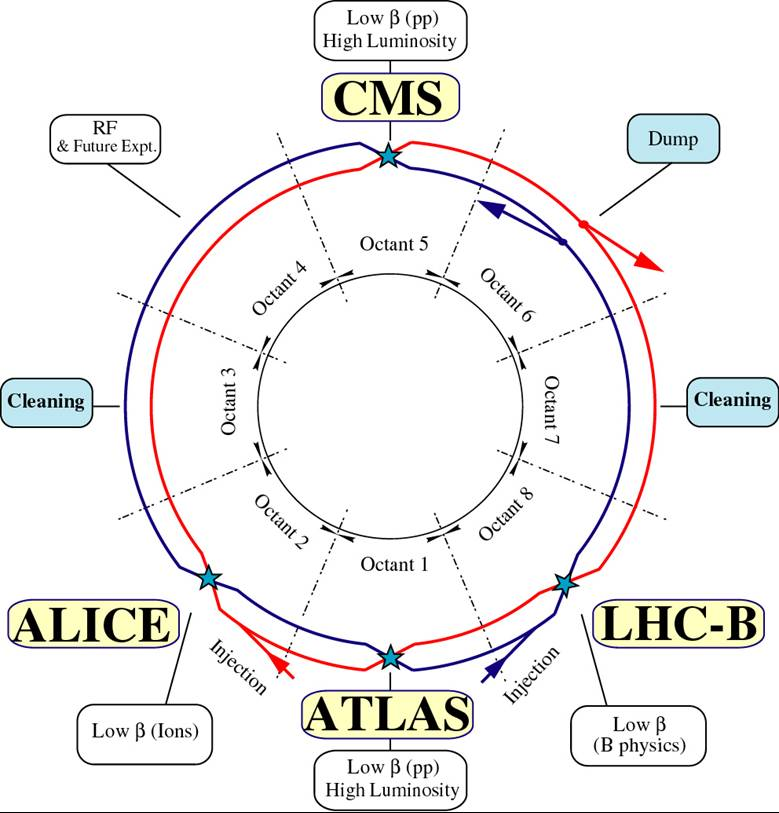
\includegraphics[width=0.8\textwidth]{./Figures/detector/lhcDiagram}
  \caption{Schematic layout of the LHC showing the position of the four main detectors as
  well as the RF systems}
  \label{fig:LHC-diagram}
\end{figure}

\subsection{LHC run condictions}

The first physics runs of the LHC from 2010-2013 (Run 1) reached energies of 3.5 and 4 TeV per beam and 
provided record-breaking integrated luminosities. The data collected allowed 
for the discovery of the higgs boson\cite{higgs} as well as enabling many new regions of parameter space
to be probed. From 2013 to mid-2015 (Long Shutdown 1) the LHC was shut down for upgrade to allow design
energies to be reached. All magnet interconnectors were inspected and replaced where necessary 
and the dipole magnets underwent a quench training programme. 

After LS1, from 2015-2016 (Run 2, which will continue up to 2018) the LHC has been running with record beam energies 
of $6.5\TeV$ per beam with bunch spacings of 25 and 50 ns. 
As shown in Figure~\ref{fig:LHC-integrated-lumi}, in 2016, $40.7\fb$ of integrated luminosity has been 
delivered to the CMS and ATLAS detectors, with $37.5\fb$ recorded by CMS. The dataset is validated by detector
subsytem experts to ensure runs in which the data quality may be affected by any problem in one of the CMS detectors 
subsystems are excluded. The luminosity of this certified dataset is XX and it is this dataset, 
at a centre of mass energy of $\sqrt(s) = 13\TeV$, 
which is used in Chapters XX to search for Supersymmetry at the highest energy reached at a collider.

%%%FIGURE - LHC lumi plot
\begin{figure}
\centering
    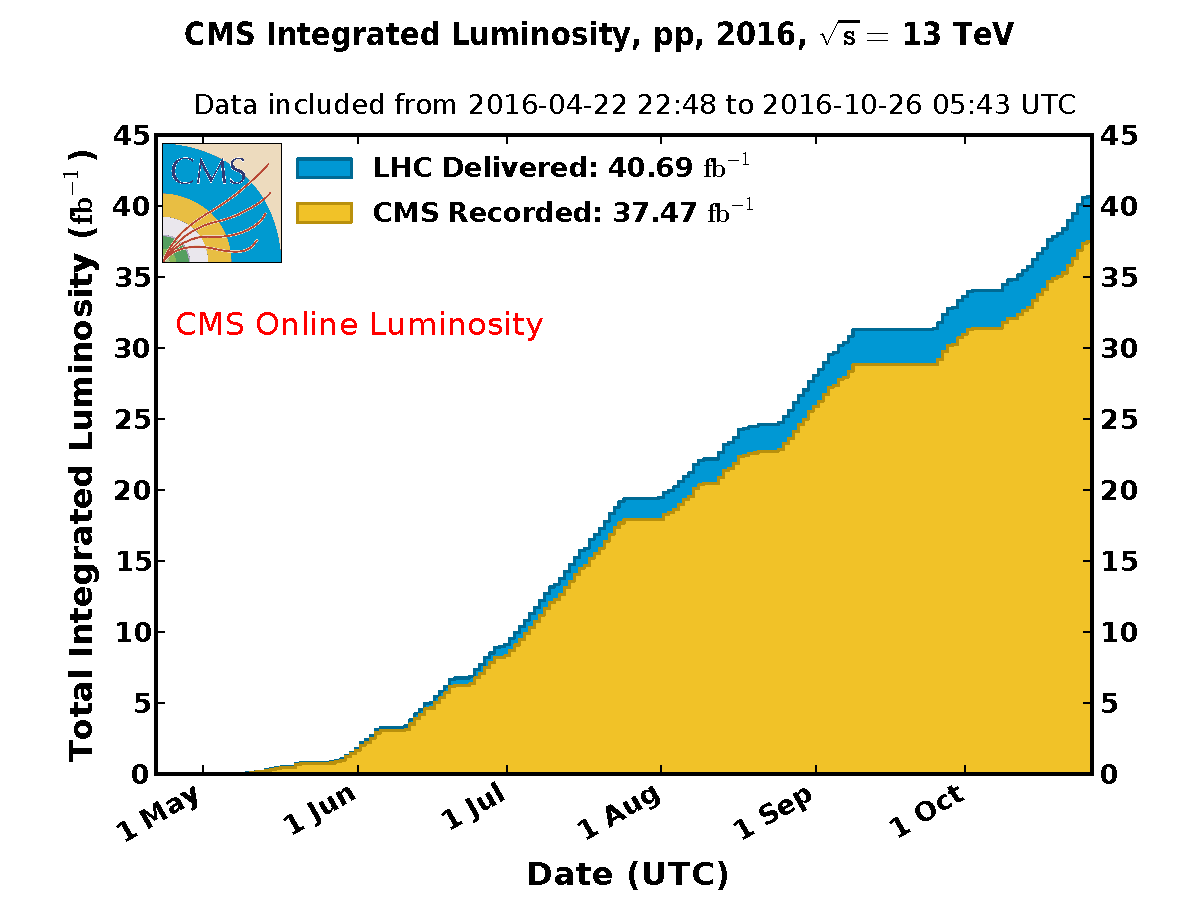
\includegraphics[width=0.9\textwidth]{./Figures/detector/int_lumi_per_day_cumulative_pp_2016OnlineLumi}
  \caption{Integrated luminosity measured online versus day delivered to (blue), 
  and recorded by CMS (orange) during stable beams and for p-p collisions at 13 TeV centre-of-mass energy in 2016.}
  \label{fig:LHC-integrated-lumi}
\end{figure}

%----------------------------------------------------------------------------------------
\section{The CMS detector}
The Compact Muon Solenoid (CMS \cite{CMS}) is one of two general purpose detectors at the LHC 
which have performed exceptionally well during the physics runs of the LHC. The main design goals
for CMS were to discover the Higgs boson as well as to search for generic models 
of new physics. To achieve this, CMS provides efficient identification and measurement
of physics objects including muons, electrons, photons, taus and hadronic showers over a
wide range of momenta and energies. Each major subsystem is made of a barrel
and two endcaps to give coverage of almost $4\pi$ in solid angle. 
This barrel design allows global momentum imbalance to be effectively 
reconstructed allowing the missing energy predicted in many new models of physics to be
precisely measured. A more detailed description may be found in \cite{CMS}.  

The coordinate system used by CMS takes the origin at 
the collision point. The z-axis points along the beam direction while the x-axis points radially inward
towards the centre of the LHC and the y-axis points vertically upward.
The polar angle, $\theta$, is measured from the z-axis and defines the psuedorapidity, $\eta=-ln(tan(\theta/2))$. 
This is used in preference to $\theta$ as the difference between the pseudorapidity of two 
particles is invarient under boosts along the z-axis. 
The eta coverage of CMS is $|\eta|<5$. The azimuthal angle, $\phi$, is defined from the x-axis in the x-y plane.
This allows the definition of $\Delta R = \sqrt(\Delta\phi^2+\Delta\eta^2)$, commonly used to measure the 
angular difference between objects. Transverse energies and momenta, $E_T $ and $p_T$ respectively, are defined \cite{cmsiop}
as $E_T = E\sin(\theta)$ and $p_T = \sqrt(p_{x}^2+p_{y}^2)$. Momentum imbalances are measured as the negative 
vector sums of the momenta of the relevant objects in the x-y plane. 

\begin{figure}
\centering
    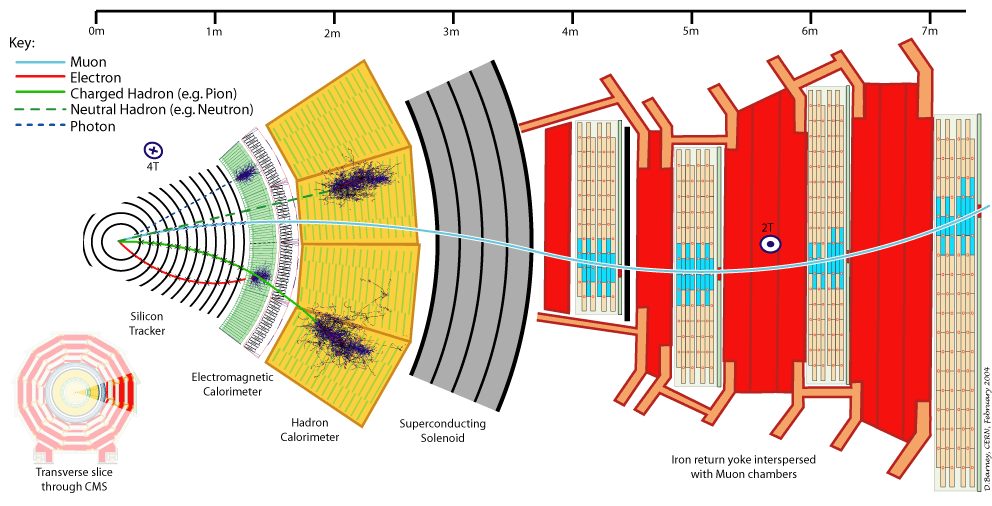
\includegraphics[width=0.9\textwidth]{./Figures/detector/CMS_Slice.jpg}
  \caption{Cross Section of CMS showing the paths of various particle types 
  through different segments of the detector \cite{cmsslice}}
  \label{CMS_SLICE}
\end{figure}

Figure \ref{CMS_SLICE} shows a cross-section of CMS in the $x-y plane$ plane as well as introducting the major detector components that will be described 
in detail in this section. The tracker lies closest to the beam and, as for the calorimetry subsystems, is situated within a magnetic field of 3.8T provided
by the superconducting solenoid. It measures the curved trajectory of charged particles through the magnetic field to determine their momenta 
as well as the location of primary and secondary vertices. The tracker is followed by the electromagnetic calorimeter (ECAL)
which measures energy deposited in electromagnetic showers from particles such as electrons and photons. The hadronic calorimeter
(HCAL) lies outside the ECAL and measures energy from nuclear interactions of hadronic particles. It is a sampling calorimeter
made up of several layers of absorber and scintillator to allow hadron showers 
to be measured over a maximum of around 11 radiation lengths. The coverage of the hadron calorimeter is extended into the 
forward regions with the forward calorimeter (HF). Enclosing the calorimeter and tracker is the superconducting solenoid. The iron return
yoke is interspersed with muon chambers which form the outermost components of the detector. Muons are minimally ionising particles (MIPs),
depositing little energy within the detector, and typically reach the surrounding cavern containting the detector. The barrel muon system
is composed of drift-tubes (DT) and resitive plate chambers (RPC), together these provide high resolution hit timing and positioning to determine
the moun trajectory. In the endcaps the DTs are replaced by cathode strip chambers (CSC) due to the higher radiation flux occuring
along the beamline. 

\subsection{Tracker}
The CMS tracker is an all-silicon tracker with a sensitive area of around 200$m^2$ to charged particles. It is designed to measure points along the
curved trajectories of charged particles resulting from the high energy p-p collisions within $\|\eta\| < 2.5$ and achieves
an optimal efficiency for the barrel region $\|\eta\| < 0.9$ \cite{tracker_performance,tracker_tdr}. A cross section of the tracker is shown in Fig~\ref{TRACKER_SLICE}.
Close to the interaction vertex ($r < 20cm$) where the particle flux is maximal ($~10^7/s$) is the pixel detector. This system consists of an inner region of 66 million silicon 
pixels of $100\mu m \times 150\mu m$ in thress overlapping layers and a forward region with two endcap discs on each side.
For r > 20cm the particle flux drops to enable the use of larger silicon microstrips. These range in size from at least $10cm \times 80\mu m$ for the Inner Barrel (TIB) region 
at intermediate values of r ($20cm < r < 55cm$) to at least $25cm \times 180\mu m$ for the Outer Barrel (TOB) region ($55cm < r < 110cm$). The forward region
for r > 20cm is covered by endcap disks divided into the 9 disks of the Tracker End Cap (TEC) for the $120cm < \|z\| Z 280 cm$ region and 
3 Tracker Inner Discs (TID) lying between the TIB and TEC. The TID and first 3 disks of the TEC have sensor thickness $320\mu m$ while the remainder of the TEC disks
have thickness $500\mu m$\cite{tracker_tdr}.

\begin{figure}
\centering
    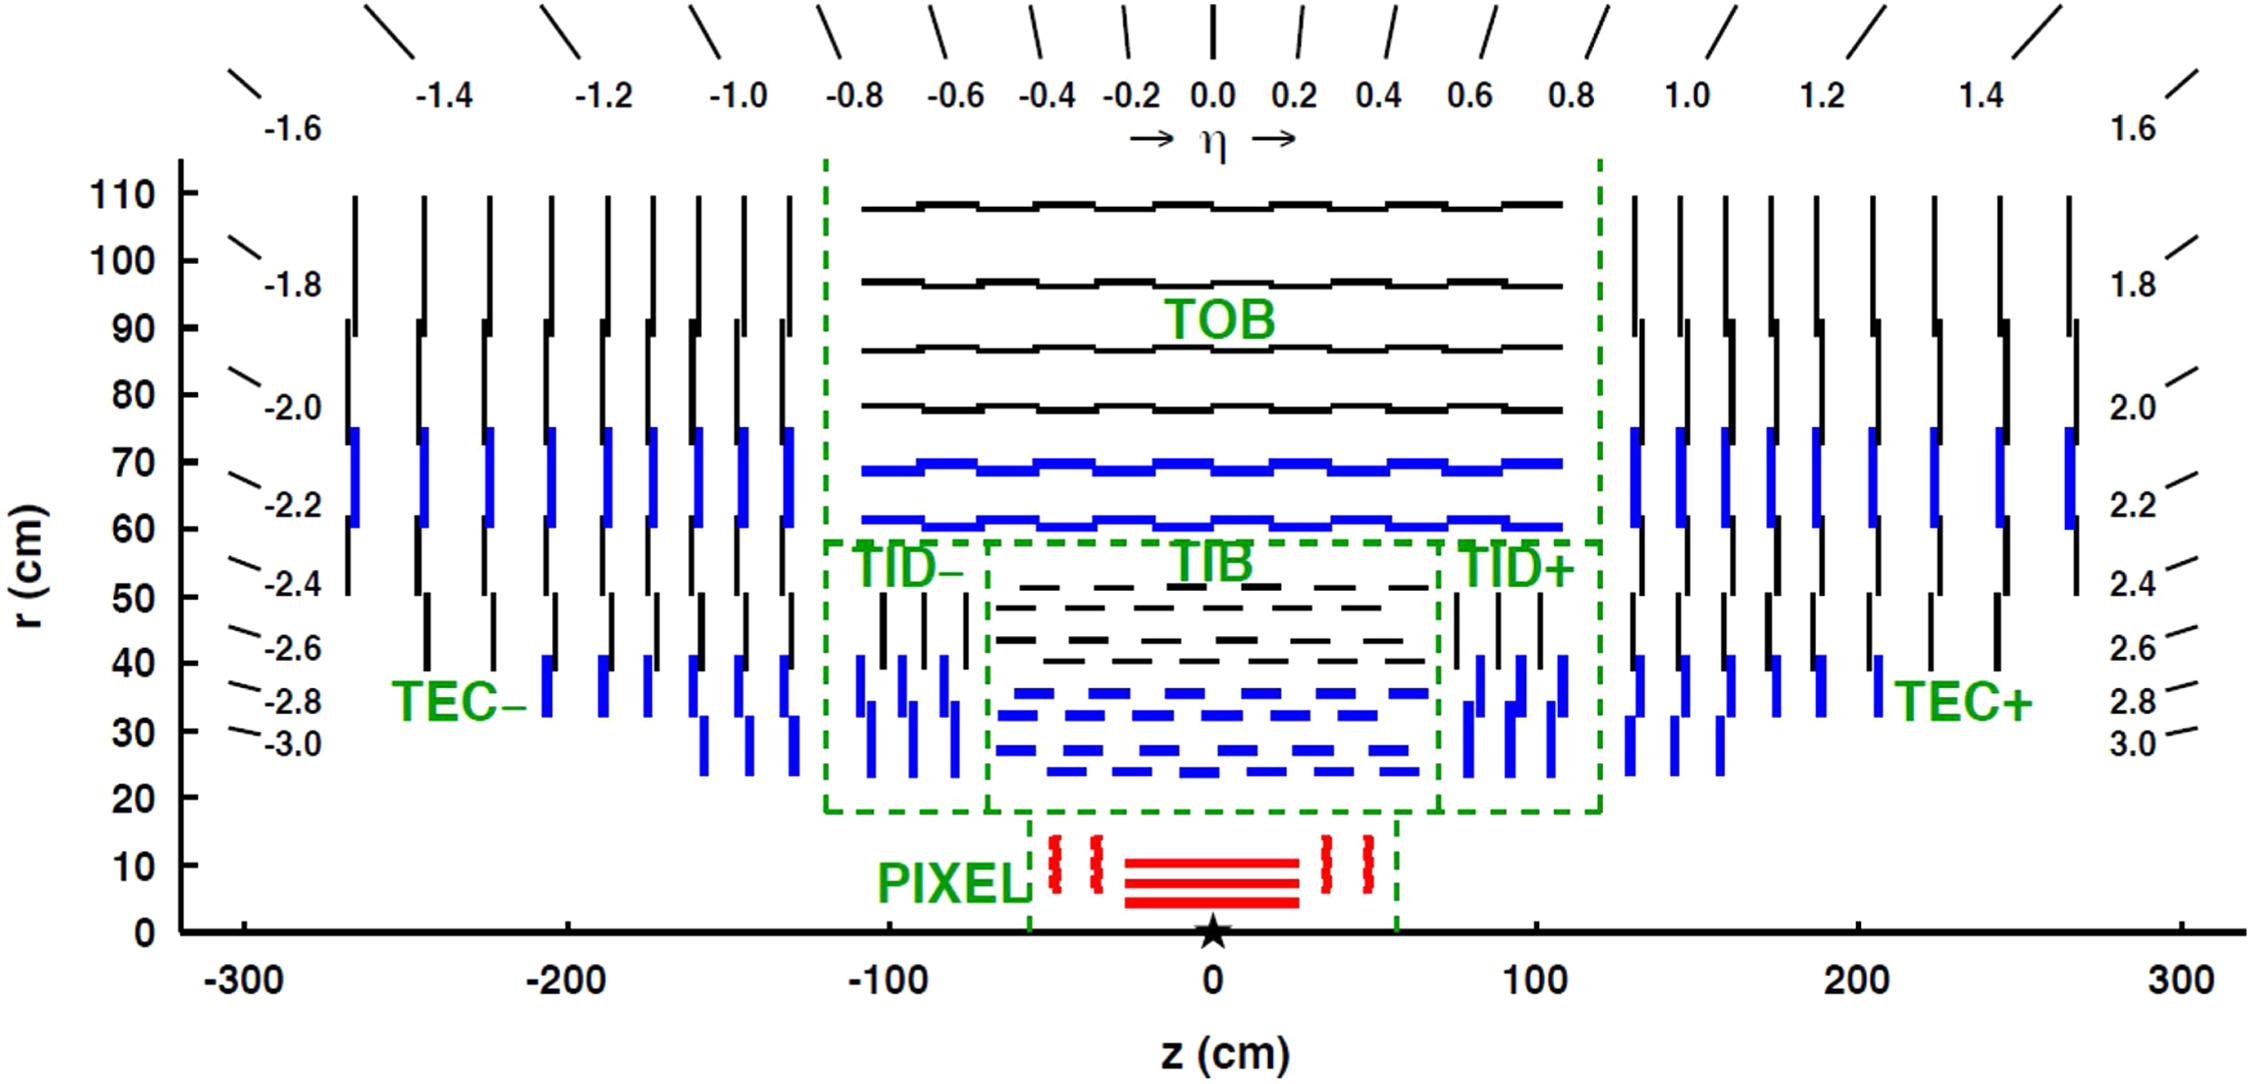
\includegraphics[width=0.9\textwidth]{./Figures/detector/CMS2Dtracker}
  \caption{A quarter cross section of the CMS tracker showing the pixel and strip components \cite{tracker_fig}}
  \label{TRACKER_SLICE}
\end{figure}

To measure the trajectories the tracker must effectively detect hits from charged particles. The efficiency for the 
hit reconstruction, defined as the fraction of particles with $p_T > 1 GeV$ passing through the fiducial regions of the sensors
in a layer for which hits are recorded, ranges from 99\% in the strip detector to 99.5\% for the pixel detector.
For the pixel detector the resolution in the r-$\phi$ plane is $\sim10\mu m$ and $\sim20-40\mu m$ along
the z direction while the r-$\phi$ resolution for the strip detector ranges from $\sim13-47\mu m$.

\subsubsection{Tracks}
Charged particle tracks are reconstructed from the hits, considering the efficiency and resolution, 
using the iterative Combinatorial Track Finder (CTF) algorithm. The track reconstruction can be decomposed 
into four logical steps outlined below.

\begin{itemize}
\item Seeds are generated using either triplets of tracker hits or pairs of hits with an additional constraint 
from the beamspot or a pixel vertex. This gives an initial estimate of the trajectory with uncertainty \cite{tracker_early}.
\item Each seed is propagated outward through the tracker layers considering the current uncertainty in the trajectory.
In propagating, a uniform magnetic field as well as no energy loss or multiple Coulomb scattering effects are assumed.
The track parameters are then updated with the best matching hit on each layer (if any) according to the Kalman filter formalism \cite{tracker_vertex}.
The search continues until either the boundary of the tracker is reached or no more compatible hits are found. If a mimimum number
of valid hits are observed an inwards search is initiated for additional hits\cite{tracker_early}.
\item It is possible for a single charged particle trackto be reconstructed more than once, starting either from different seeds or if
one seed develops into multiple track candidates. If the fraction of shared hits between two track candidates is greater
than 19\% (determined empically) the track with fewer hits is discarded. If the number of hits is equivalent the track with
 the largest $\chi^2$ is discarded\cite{tracker_vertex}.
\item After the track candidates are built and cleaned the hits in each candidate are refitted using a Kalman filter and smoother. This 
avoids possible bias from the seeding stage \cite{tracker_vertex}.
\end{itemize}

The CTF performs six iterations to determine the tracks. Between each iteration any hits that are assigned to tracks in the
previous iteration are removed from the collection. The final track collection is then filtered to remove fake tracks using 
information on the number of hits, the $chi^2$ and the compatibilty of the track orginating from a pixel vertex. The momentum 
resolution achieved is 0.7 (5)\% at 1 (1000) \GeV in the central region\cite{tracker_early}. Using a dataset of pions and muons data from an early run 
at the LHC the tracking efficiency was measured as 98\% for tracks with $p_T > 500\MeV$ and $>99\%$ for tracks with $p_T > 2\GeV$\cite{tracker_eff}.

\subsubsection{Vertex Reconstruction}

As described in Sec.~\ref{lhc_intro}, the LHC produced an average of 25 simultaneous collisions per bunch crossing
during Run 2. It is essential to identify the Primary Vertex (PV) and the particles originating from it to allow 
particles from additional collisions to be rejected and to identify features such as displaced vertices. The tracks
are initally clustered using a deterministic annealing (DA) algorithm based on the points of closest approach of the 
tracks to the beamspot\cite{tracker_vertex}. The candidate vertices containing at least two tracks are then
fitted using an adaptive vertex fitter to compute the best estimates of vertex parameters\cite{tracker_avf}. 
Each track in the vertex is assigned a weight between 0 and 1 corresponding to the likelihood that that track
belongs to the vertex. The tracks with weight near 1 are most consistent with the reconstructed vertex while
those that are least consistent have small weights. The number of degrees in the fit is an important parameter
for distinguishing real proton-proton interactions from misclustered vertices as it is strongly corrected with
the number of tracks compatible with arising from the interaction region\cite{tracker_vertex} and is defined 
as

\begin{equation}
n_{dof} = -3 + 2 \sum_{i=1}^{\#tracks} wi,
\end{equation}
The vertex position and resolution have been measured in early LHC data and compared with simulation as shown in 
Fig~\ref{fig:pvEffRes}.

\begin{figure}[hbt]
  \begin{center} 
   \subfigure[\label{fig:pvEff}]{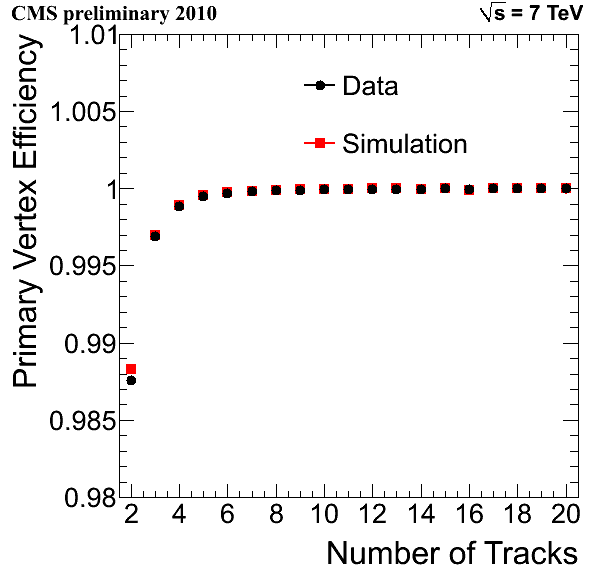
\includegraphics[width=0.5\textwidth]{Figures/detector/pvEff}}~
   \subfigure[\label{fig:pvRes}]{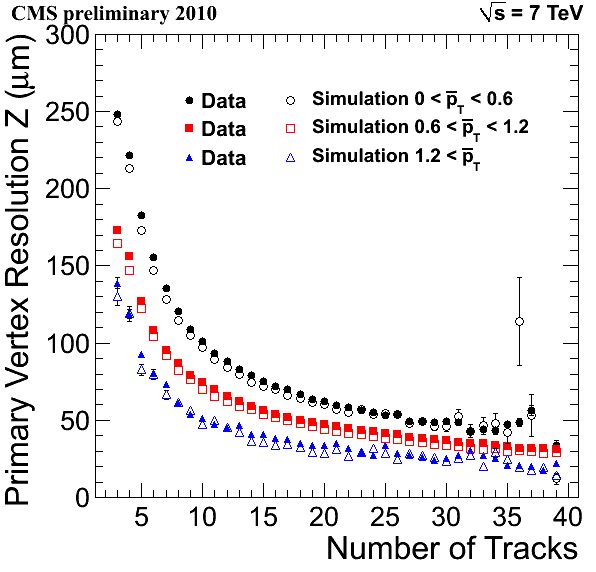
\includegraphics[width=0.5\textwidth]{Figures/detector/pvRes}}
   \caption{(a) Primary Vertex efficiency as a function of the number of associated tracks. (b) Primary Vertex 
   resolution in the z coordinate as a function of the number of associated tracks for three track $p_T$ scenarios \cite{tracker_seven}
   \label{fig:pvEffRes} }
  \end{center}
\end{figure}
The vertices are ordered according to the sum of the $p_T^2$ of the tracks associated to each vertex with the 
vertex with the highest $p_T^2$ taken as the primary vertex (PV). The position of the primary vertex can
be used for object identification and control of pile-up. Many CMS analyses, including the one in this 
thesis, make requirements that a good vertex is reconstructed from the tracks satisfying:

\begin{itemize}
\item A minimum number of degrees of freedom: $n_{dof} > 4$.
\item The collision to occur with $|z| < 24cm$ such that the primary vertex is near the interaction point in the longitudinal direction
\item The collision to occur within a radial distance of $|d_{xy}| < 24cm$ from the beamline 
\end{itemize}
% The primary vertex is reconstructed using the deterministic annealing (DA) clustering algorithm which selects tracks
% based on their compatibilty with the beam spot, number of hits and fit quality and clusters them into several primary
% vertex candidates. 

% \begin{description}
% \item[Silicon Tracker]The job of the tracker is to measure the momentum of charged particles from their path through a magnetic field \cite{siliconTDR}. The CMS tracker achieves $10\mu m$ accuracy with coverage for $|\eta|<2.5$ and has a resolution of 1\%.
% \item[Electromagnetic Calorimeter (ECAL)] The ECAL measures the energy of incident photons and electrons. The ECAL barrel is made of 61,200 $PbWO_4$ crystals and provides coverage for $|\eta|<1.48$ \cite{ecal}. This is extended to $|\eta|<3$ by the endcap which adds another $10764$ crystals. The endcap has a pre-shower to distinguish between $\gamma$ and $\pi^0$. The ECAL has a resolution of 0.5\%.
%  \item[Hadronic Calorimeter (HCAL)] The HCAL is made from alternating brass and scintilator layers with a coverage of $|\eta|<3.0$ \cite{hcal}. The coverage is extended to  $|\eta|<5.0$ by an iron/quartz forward calorimeter \cite{hfhcal}. The average resolution is 11\%. 
%  \item[Muon Chambers]The muons are not stopped by any of the calorimeters and therefore require a separate detector with coverage $|\eta| < 2.4$. The muon chambers are interspersed with the magnet return yoke. The high magnetic field allows for accurate momentum measurement \cite{muons}. The resolution is 1\%.
% \end{description}
% As the data rate ($40Mhz$) is far too high for every event to be stored and as new physics will only 
% be seen in a minority of events a trigger system for interesting events is necessary. 
% This happens in two stages: the L1 Calorimetric and Muon Trigger (Hardware) and the High Level Trigger (Software) \cite{HLT}. 
% The L1 trigger must operate within $\mathcal{O}10ns$ and so  the calorimetric trigger only takes input
% from the ECAL and HCAL. This is described in more detail in chapter \ref{Chapter3}. The input from the
% L1 triggers is then combined in the Global Trigger (GT) which decides whether to keep the event. 
% The $\mathcal{O}100kHz$ events which pass L1 selection are processed in the HLT which utilises the 
% calorimeter information along with tracking and the muon system to further reduce the rate to $\mathcal{O}1kHz$.
